\chapter{अम्ल और क्षारक: Ka और pKa}\label{ch:g12:ka-and-pka}

अनेक चींटियाँ मेथेनोइक अम्ल से अपनी रक्षा करती हैं, और त्वचा पर यह
जलन पैदा करता है। मेथेनोइक अम्ल एक छोटा
\omterm{def:g11:functional-groups:carboxylic-acid}{कार्बोक्सिलिक अम्ल} है। उसी सांद्रता पर हाइड्रोक्लोरिक अम्ल कहीं
अधिक जलाता। दोनों अम्ल हैं; दोनों 7 से कम \omterm{def:g9:acids-bases-ph:ph}{pH} वाला विलयन देते हैं; फिर भी वे
एक ही ढंग से अम्लीय नहीं हैं। किसी अम्ल का पूरा वर्णन करने के लिए दो संख्याएँ
चाहिए: उसकी कितनी मात्रा है, यानी उसकी सांद्रता, और वह कितनी आसानी से
अपना हाइड्रोजन \omterm{def:g9:ions:ion}{आयन} दे देता है, यानी उसका \omterm{def:g12:ka-and-pka:ka}{अम्लता स्थिरांक}।

\begin{recall}
अम्लीय, क्षारकीय और \omterm{def:g9:acids-bases-ph:acidic}{उदासीन विलयन}; \omterm{def:g9:acids-bases-ph:ph}{pH} पैमाना, 0 से 14 तक, जो
हाइड्रोजन \omterm{def:g9:ions:ion}{आयन} अधिक होने पर कम होता है (\cref{ch:g9:acids-bases-ph})।
\omterm{def:g12:equilibrium:quotient}{अभिक्रिया भागफल} $Q$ और \omterm{def:g12:equilibrium:constant}{साम्य स्थिरांक} $K$
(\cref{ch:g12:equilibrium})। \omterm{def:g12:curly-arrows:curly-arrow}{वक्र तीर} \omterm{def:g9:inside-the-atom:nucleus}{इलेक्ट्रॉनों} के एक युग्म की
गति दिखाता है (\cref{ch:g12:curly-arrows})।
\end{recall}

\begin{omfigure}
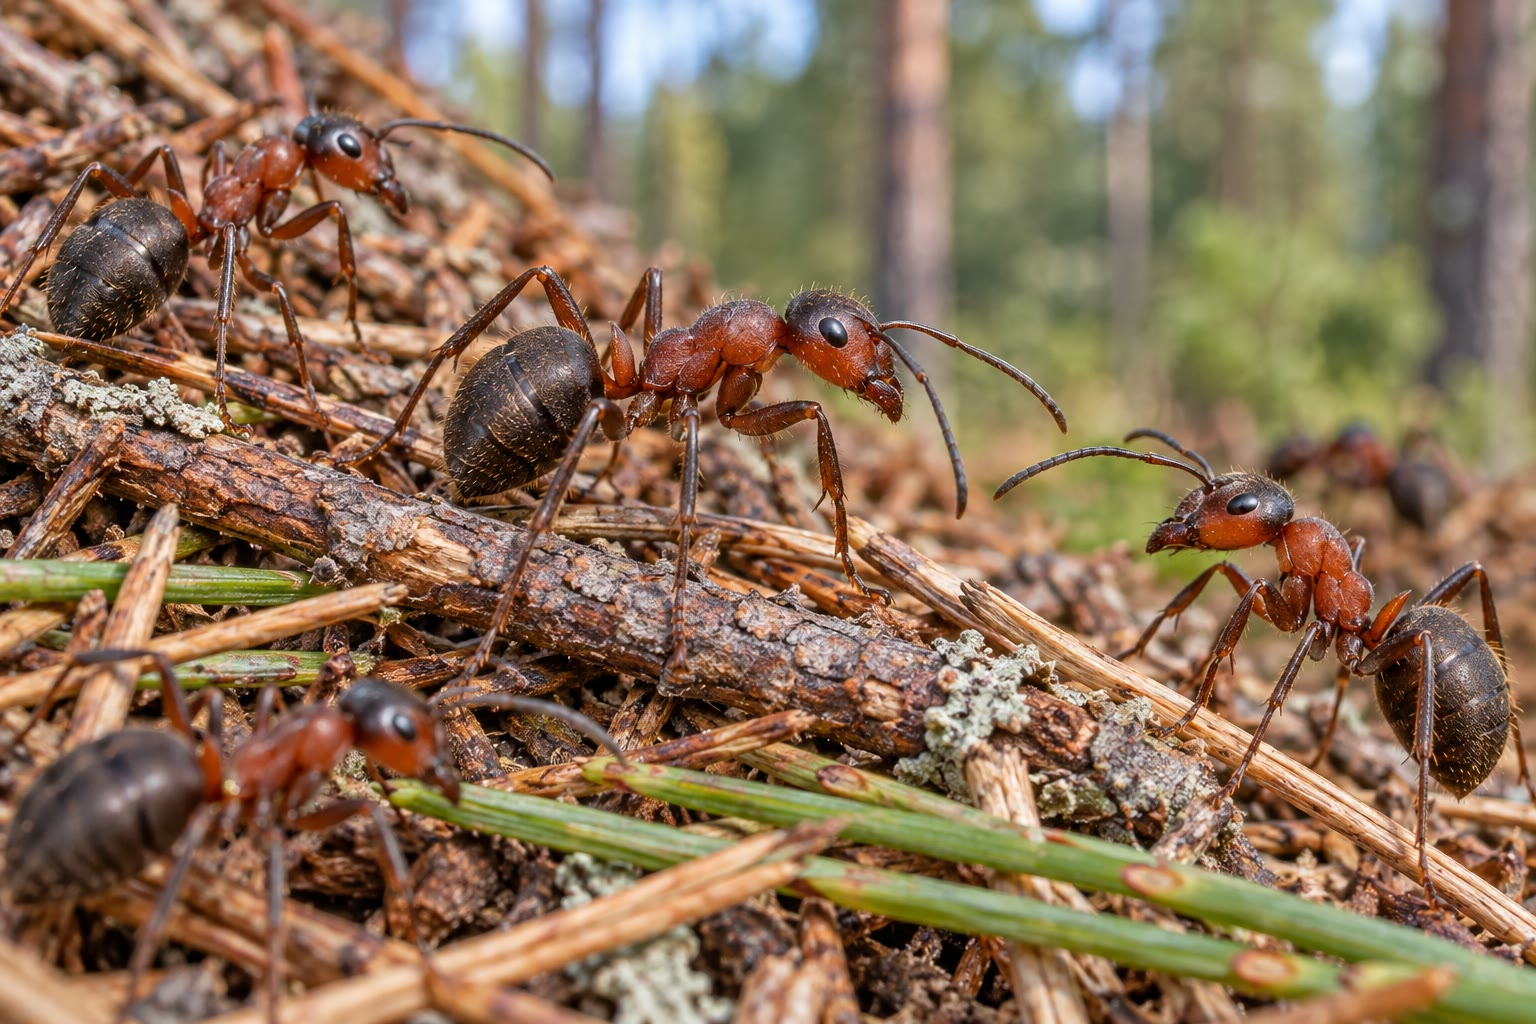
\includegraphics[width=0.45\linewidth]{images/book1/ai/g12-red-ants.jpg}

{\small जंगल की लाल चींटियाँ: अनेक चींटियों की तरह वे मेथेनोइक अम्ल से अपनी रक्षा करती हैं।}
\end{omfigure}

\section{ब्रॉन्स्टेड अम्ल और क्षारक}

\begin{definition}[ब्रॉन्स्टेड अम्ल और क्षारक, अम्ल--क्षारक युग्म]\label{def:g12:ka-and-pka:bronsted}
\emph{ब्रॉन्स्टेड अम्ल}\index{ब्रॉन्स्टेड अम्ल} वह स्पीशीज़ है जो
हाइड्रोजन \omterm{def:g9:ions:ion}{आयन} \ce{H+} दे सकती है; \emph{ब्रॉन्स्टेड क्षारक}\index{ब्रॉन्स्टेड क्षारक} वह
स्पीशीज़ है जो उसे ले सकती है। अम्ल HA और वह क्षारक \ce{A-} जो वह
\ce{H+} खोकर बनता है, मिलकर एक \emph{अम्ल--क्षारक युग्म}\index{अम्ल--क्षारक युग्म} बनाते हैं,
जिसे \ce{HA}/\ce{A-} लिखा जाता है: $\ce{HA} \rightleftharpoons \ce{A-} + \ce{H+}$।
\end{definition}

\begin{definition}[ऑक्सोनियम आयन, उभयधर्मी]\label{def:g12:ka-and-pka:oxonium}
पानी में हाइड्रोजन \omterm{def:g9:ions:ion}{आयन} कभी अकेला नहीं रहता: उसे पानी का एक
\omterm{def:g7:atoms-and-molecules:molecule}{अणु} ले लेता है, जिससे \emph{ऑक्सोनियम आयन}\index{ऑक्सोनियम आयन} \ce{H3O+} बनता है।
जो स्पीशीज़ एक युग्म का अम्ल और दूसरे का क्षारक हो, वह
\emph{उभयधर्मी}\index{उभयधर्मी} है; पानी ऐसा ही है, युग्म
\ce{H2O}/\ce{OH-} का अम्ल और युग्म \ce{H3O+}/\ce{H2O} का क्षारक।
\end{definition}

\begin{example}[पानी में एक अम्ल]\label{ex:g12:ka-and-pka:acid-water}
जब एथेनोइक अम्ल \omterm{def:g2:mixing-and-dissolving:dissolve}{घुलता} है, तो पानी के एक \omterm{def:g7:atoms-and-molecules:molecule}{अणु} का \omterm{def:g10:lewis-and-shape:lone-pair}{एकाकी युग्म} उसके
\ce{O-H} का हाइड्रोजन ले लेता है, और \ce{O-H} युग्म अम्ल के ऑक्सीजन पर ही रह जाता है:
\[
  \ce{CH3COOH + H2O <=> CH3COO- + H3O+} .
\]
दो युग्म एक हाइड्रोजन \omterm{def:g9:ions:ion}{आयन} का आदान-प्रदान करते हैं: \ce{CH3COOH}/\ce{CH3COO-} उसे देता है,
\ce{H3O+}/\ce{H2O} उसे लेता है। अब से, जब भी पानी \omterm{def:g6:solutions-and-solubility:solute}{विलायक} हो, पहले के
अध्यायों के हाइड्रोजन \omterm{def:g9:ions:ion}{आयन} \ce{H3O+} लिखे जाएँगे।
\end{example}

\begin{omfigure}
\setchemfig{atom sep=2em}
\chemfig{H_3C-C(=[2]O)-O-[@{oh}]@{h}H}\qquad
\chemfig{@{ow}\charge{90=\:,270=\:}{O}(-[:150]H)-[:210]H}
\qquad$\longrightarrow$\qquad
\chemfig{H_3C-C(=[2]O)-\charge{90=\:,0=\:,270=\:}{O}^{-}}\quad$+$\quad\ce{H3O+}
\chemmove{
  \draw[->, thick, omProp, shorten <=4pt, shorten >=3pt]
    ($(ow)+(0,0.25)$) .. controls +(110:9mm) and +(60:9mm) .. (h);
  \draw[->, thick, omDef, shorten <=2pt, shorten >=4pt]
    (oh) .. controls +(-90:7mm) and +(-60:6mm) .. ($(oh)+(-0.3,-0.2)$);}

{\small एक हाइड्रोजन \omterm{def:g9:ions:ion}{आयन} अम्ल से पानी में जाता है: पानी का एक \omterm{def:g10:lewis-and-shape:lone-pair}{एकाकी युग्म}
नया \ce{O-H} आबंध बनाता है (नारंगी), और पुराना \ce{O-H} युग्म
एथेनोएट \omterm{def:g9:ions:ion}{आयन} के ऑक्सीजन पर रह जाता है (नीला)।}
\end{omfigure}

\begin{history}[आरेनियस से ब्रॉन्स्टेड तक, 1887--1923]
1887 में स्वांते आरेनियस ने प्रस्ताव रखा कि अम्ल पानी में हाइड्रोजन \omterm{def:g9:ions:ion}{आयन} देते हैं
और क्षारक हाइड्रॉक्साइड \omterm{def:g9:ions:ion}{आयन}। 1923 में योहानेस ब्रॉन्स्टेड ने, और स्वतंत्र रूप से
थॉमस लोरी ने, इस विचार को व्यापक बनाया: अम्ल वह कोई भी स्पीशीज़ है जो
हाइड्रोजन \omterm{def:g9:ions:ion}{आयन} देती है, क्षारक वह कोई भी स्पीशीज़ जो उसे लेती है, पानी में हो या न हो।
अमोनिया का \omterm{def:g7:atoms-and-molecules:molecule}{अणु}, जिसमें कोई हाइड्रॉक्साइड नहीं, अन्य क्षारकों की तरह ही
एक क्षारक बन गया।
\end{history}

\begin{omfigure}
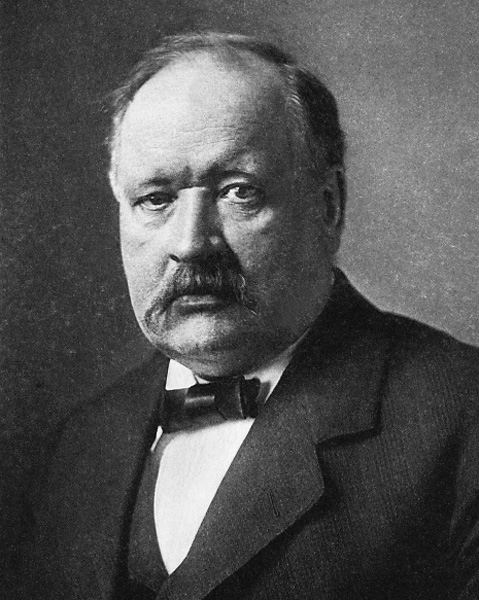
\includegraphics[width=0.22\linewidth]{images/book1/arrhenius.jpg}

{\small स्वांते आरेनियस (1859--1927)।}
\end{omfigure}

\section{pH, मात्रात्मक रूप से}

\begin{definition}[pH, सटीक रूप से]\label{def:g12:ka-and-pka:ph-log}
किसी तनु \omterm{def:g6:solutions-and-solubility:solute}{जलीय विलयन} में \omterm{def:g9:acids-bases-ph:ph}{pH} इस प्रकार परिभाषित है:
\[
  \mathrm{pH} = -\log\frac{[\ce{H3O+}]}{c^\circ},
  \qquad\text{अर्थात}\qquad
  [\ce{H3O+}] = c^\circ \times 10^{-\mathrm{pH}} ,
\]
जहाँ $\log$ दाशमिक लघुगणक है।
\end{definition}

\begin{proposition}[दस गुना तनुकरण, एक इकाई]\label{prop:g12:ka-and-pka:dilution}
यदि $[\ce{H3O+}]$ को 10 से विभाजित किया जाए, तो \omterm{def:g9:acids-bases-ph:ph}{pH} 1 बढ़ जाता है; यदि उसे
10 से गुणा किया जाए, तो \omterm{def:g9:acids-bases-ph:ph}{pH} 1 घट जाता है।
\end{proposition}

\begin{proof}
$-\log\big([\ce{H3O+}]/10c^\circ\big) = -\log\big([\ce{H3O+}]/c^\circ\big)
+ \log 10 = \mathrm{pH} + 1$।
\end{proof}

\begin{definition}[प्रबल और दुर्बल अम्ल और क्षारक]\label{def:g12:ka-and-pka:strong-acid}
\emph{प्रबल अम्ल}\index{प्रबल अम्ल} पानी से पूर्ण रूप से अभिक्रिया करता है: विलयन में
अम्ल का कुछ भी अपने मूल रूप में नहीं बचता। \emph{दुर्बल
अम्ल}\index{दुर्बल अम्ल} आंशिक रूप से अभिक्रिया करता है: पानी के साथ उसकी अभिक्रिया
एक साम्य तक पहुँचती है। इसी प्रकार \emph{प्रबल क्षारक}\index{प्रबल क्षारक} पानी से
पूर्ण रूप से अभिक्रिया करता है, \emph{दुर्बल क्षारक}\index{दुर्बल क्षारक} आंशिक रूप से।
\end{definition}

\begin{proposition}[प्रबल अम्ल का pH]\label{prop:g12:ka-and-pka:strong}
सांद्रता $c$ (बहुत तनु नहीं) वाले \omterm{def:g12:ka-and-pka:strong-acid}{प्रबल अम्ल} के विलयन में
$[\ce{H3O+}] = c$ और $\mathrm{pH} = -\log(c/c^\circ)$ होता है।
\end{proposition}

\begin{proof}
अभिक्रिया \ce{HA + H2O -> A- + H3O+} पूर्ण है: अम्ल का हर \omterm{def:g7:atoms-and-molecules:molecule}{अणु}
एक \omterm{def:g12:ka-and-pka:oxonium}{ऑक्सोनियम आयन} देता है। स्वयं पानी से आने वाले \omterm{def:g9:ions:ion}{आयन} नगण्य हैं
जब तक $c$ \qty{e-7}{mol/L} से बहुत बड़ा है।
\end{proof}

\begin{example}[हाइड्रोक्लोरिक अम्ल]\label{ex:g12:ka-and-pka:hcl}
\qty{0.010}{mol/L} पर हाइड्रोक्लोरिक अम्ल: $[\ce{H3O+}] = \qty{0.010}{mol/L}$
और $\mathrm{pH} = -\log 0.010 = 2.0$। दस गुना तनु करने पर \omterm{def:g9:acids-bases-ph:ph}{pH} 3.0।
\end{example}

\section{पानी और आयनिक गुणनफल}


\begin{definition}[जल का आयनिक गुणनफल]\label{def:g12:ka-and-pka:ionic-product}
पानी स्वयं से बहुत थोड़ी अभिक्रिया करता है, \ce{2H2O <=> H3O+ + OH-}। इस
अभिक्रिया का \omterm{def:g12:equilibrium:constant}{साम्य स्थिरांक} \emph{जल का आयनिक
गुणनफल}\index{जल का आयनिक गुणनफल} है:
\[
  K_e = \frac{[\ce{H3O+}]\,[\ce{OH-}]}{(c^\circ)^2},
  \qquad pK_e = -\log K_e .
\]
\end{definition}

\begin{proposition}[उदासीन पानी और प्रबल क्षारक]\label{prop:g12:ka-and-pka:ke}
% ledger: ke:25C
\qty{25}{\celsius} पर $K_e = \num{1.0e-14}$ और $pK_e = 14.0$। शुद्ध
पानी में $[\ce{H3O+}] = [\ce{OH-}] = \qty{1.0e-7}{mol/L}$: \omterm{def:g9:acids-bases-ph:ph}{pH} 7.0। सांद्रता $c$
वाला \omterm{def:g12:ka-and-pka:strong-acid}{प्रबल क्षारक} $[\ce{OH-}] = c$ देता है, इसलिए
$[\ce{H3O+}] = K_e (c^\circ)^2 / c$ और $\mathrm{pH} = 14.0 + \log(c/c^\circ)$।
\end{proposition}

\begin{proof}
शुद्ध पानी में दोनों \omterm{def:g9:ions:ion}{आयन} जोड़ों में आते हैं, इसलिए वे बराबर हैं, और उनका
गुणनफल $\num{1.0e-14}$ है: हर एक \qty{1.0e-7}{mol/L} है। क्षारक के लिए,
विलयन में $K_e$ अब भी लागू रहता है:
$-\log([\ce{H3O+}]/c^\circ) = -\log K_e + \log(c/c^\circ)$।
\end{proof}

\begin{example}[सोडियम हाइड्रॉक्साइड]\label{ex:g12:ka-and-pka:naoh}
\qty{0.010}{mol/L} सांद्रता वाला सोडियम हाइड्रॉक्साइड: इसमें $[\ce{OH-}] = 0.010$, इसलिए
$[\ce{H3O+}] = \num{1.0e-14}/0.010 = \qty{1.0e-12}{mol/L}$ और \omterm{def:g9:acids-bases-ph:ph}{pH} 12.0।
\end{example}

\section{अम्लता स्थिरांक}

\begin{definition}[अम्लता स्थिरांक, $pK_a$]\label{def:g12:ka-and-pka:ka}
किसी युग्म \ce{HA}/\ce{A-} का \emph{अम्लता स्थिरांक}\index{अम्लता स्थिरांक} $K_a$
पानी के साथ अम्ल की अभिक्रिया, \ce{HA + H2O <=> A- + H3O+}, का
\omterm{def:g12:equilibrium:constant}{साम्य स्थिरांक} है:
\[
  K_a = \frac{[\ce{A-}]\,[\ce{H3O+}]}{[\ce{HA}]\,c^\circ} .
\]
युग्म का \emph{pKa}\index{pKa} है
$pK_a = -\log K_a$।
\end{definition}

\begin{proposition}[$pK_a$ जितना छोटा, अम्ल उतना प्रबल]\label{prop:g12:ka-and-pka:compare}
समान सांद्रता वाले दो \omterm{def:g12:ka-and-pka:strong-acid}{दुर्बल अम्लों} में से, जिसका
$K_a$ बड़ा है, यानी $pK_a$ छोटा है, वह पानी से अधिक अभिक्रिया करता है और
कम \omterm{def:g9:acids-bases-ph:ph}{pH} देता है; उसका संयुग्मी क्षारक अधिक दुर्बल होता है।
\end{proposition}

\begin{proof}
बड़े $K_a$ का अर्थ है साम्य पर अधिक \ce{A-} और \ce{H3O+}, उसी \ce{HA} के लिए।
जो युग्म अपना हाइड्रोजन \omterm{def:g9:ions:ion}{आयन} आसानी से छोड़ देता है, उसका क्षारक \ce{A-}
उसे अनिच्छा से वापस लेता है।
\end{proof}

\begin{omfigure}
\begin{tikzpicture}[font=\small, y=0.55cm]
  % ledger: pka:methanoic, pka:ethanoic, pka:benzoic, pka:ascorbic1, ka:HF, ka:H2CO3, ka:HCO3, kb:NH3, ke:25C
  \draw[->, thick] (0,0) -- (0,14.8) node[above] {$pK_a$};
  \foreach \k in {0,2,4,6,8,10,12,14} \draw (-0.1,\k) -- (0.1,\k) node[right, font=\scriptsize] {\k};
  \node[font=\footnotesize\bfseries, anchor=south] at (-3.0,14.3) {अम्ल};
  \node[font=\footnotesize\bfseries, anchor=south] at (3.0,14.3) {क्षारक};
  \foreach \p/\yl/\acid/\base in {3.19/2.9/{\ce{HF}}/{\ce{F-}},
      3.74/3.6/{\ce{HCOOH}}/{\ce{HCOO-}}, 4.04/4.3/{ऐस्कॉर्बिक अम्ल}/{ऐस्कॉर्बेट},
      4.20/5.0/{\ce{C6H5COOH}}/{\ce{C6H5COO-}}, 4.76/5.7/{\ce{CH3COOH}}/{\ce{CH3COO-}},
      6.37/6.9/{\ce{CO2,H2O}}/{\ce{HCO3-}}, 9.26/9.26/{\ce{NH4+}}/{\ce{NH3}},
      10.33/10.4/{\ce{HCO3-}}/{\ce{CO3^{2-}}}} {
    \draw[omDef] (-0.25,\p) -- (0.25,\p);
    \draw[black!40] (-0.25,\p) -- (-1.1,\yl);
    \draw[black!40] (0.25,\p) -- (1.1,\yl);
    \node[anchor=east, font=\scriptsize] at (-1.15,\yl) {\acid};
    \node[anchor=west, font=\scriptsize] at (1.15,\yl) {\base};
  }
  \draw[->, omThm, thick] (-4.6,13) -- (-4.6,1);
  \node[omThm, rotate=90, font=\footnotesize] at (-4.95,7) {अधिक प्रबल अम्ल};
  \draw[->, omMeth, thick] (4.6,1) -- (4.6,13);
  \node[omMeth, rotate=90, font=\footnotesize] at (4.95,7) {अधिक प्रबल क्षारक};
\end{tikzpicture}

{\small \qty{25}{\celsius} पर अपने $pK_a$ के अनुसार रखे गए कुछ युग्म, अम्ल
बाईं ओर, उनके क्षारक दाईं ओर। पैमाने पर कोई युग्म जितना नीचे हो,
उसका अम्ल उतना ही प्रबल; जितना ऊपर, उसका क्षारक उतना ही प्रबल।}
\end{omfigure}


\begin{method}[दुर्बल अम्ल का pH]\label{met:g12:ka-and-pka:weak}
सांद्रता $c$ और स्थिरांक $K_a$ वाले \omterm{def:g12:ka-and-pka:strong-acid}{दुर्बल अम्ल} के लिए:
\begin{enumerate}
  \item प्रति लीटर \ce{HA + H2O <=> A- + H3O+} की \omterm{def:g10:reaction-progress-table:extent}{प्रगति सारणी} लिखिए,
        $x = [\ce{H3O+}]$ के साथ: $[\ce{HA}] = c - x$, $[\ce{A-}] = x$
        (पानी के अपने \omterm{def:g9:ions:ion}{आयन} नगण्य मानकर)।
  \item $\dfrac{x^2}{(c - x)\,c^\circ} = K_a$ हल कीजिए, यानी द्विघात समीकरण
        $x^2 + K_a c^\circ x - K_a c^\circ c = 0$, धनात्मक
        मूल रखते हुए।
  \item $\mathrm{pH} = -\log(x/c^\circ)$; जाँचिए कि $x$
        \qty{e-7}{mol/L} से बहुत बड़ा है।
\end{enumerate}
\end{method}

\begin{example}[\texorpdfstring{\qty{0.010}{mol/L}}{0.010 mol/L} पर एथेनोइक अम्ल]\label{ex:g12:ka-and-pka:acetic}
% ledger: pka:ethanoic
$pK_a = 4.76$, इसलिए $K_a = 10^{-4.76} = \num{1.74e-5}$। तब
$x^2 + \num{1.74e-5}\,x - \num{1.74e-7} = 0$ से
$x = \qty{4.1e-4}{mol/L}$ और \omterm{def:g9:acids-bases-ph:ph}{pH} 3.39 मिलता है। अम्ल का केवल $\num{4.1e-4}/0.010 =
\qty{4.1}{\percent}$ ही पानी से अभिक्रिया कर पाया है; उसी सांद्रता पर
हाइड्रोक्लोरिक अम्ल, \omterm{def:g9:acids-bases-ph:ph}{pH} 2.0, पूरी तरह अभिक्रिया कर चुका है।
\end{example}

\begin{omfigure}
\begin{tikzpicture}[font=\small]
  \fill[omThm!45] (0,1.3) rectangle (8,2.0);
  \node[anchor=east] at (-0.1,1.65) {\ce{HCl}, \qty{0.010}{mol/L}};
  \node[white, font=\small\bfseries] at (4,1.65) {\ce{H3O+} + \ce{Cl-}: \qty{100}{\percent}};
  \fill[omDef!35] (0,0) rectangle (7.67,0.7);
  \fill[omThm!45] (7.67,0) rectangle (8,0.7);
  \node[anchor=east] at (-0.1,0.35) {\ce{CH3COOH}, \qty{0.010}{mol/L}};
  \node at (3.8,0.35) {मूल रूप में बचा \ce{CH3COOH}: \qty{95.9}{\percent}};
  \draw[<-, omThm] (7.85,0.75) -- (8.4,1.1) node[right, font=\footnotesize] {\qty{4.1}{\percent} आयनित};
\end{tikzpicture}

{\small समान सांद्रता पर एक प्रबल और एक \omterm{def:g12:ka-and-pka:strong-acid}{दुर्बल अम्ल} का क्या होता है:
\omterm{def:g12:ka-and-pka:strong-acid}{प्रबल अम्ल} पूरी तरह \omterm{def:g9:ions:ion}{आयनों} में बदल जाता है, \omterm{def:g12:ka-and-pka:strong-acid}{दुर्बल
अम्ल} लगभग बिल्कुल नहीं। इसीलिए \omterm{def:g9:acids-bases-ph:ph}{pH} का अंतर, 2.0 के मुक़ाबले 3.4।}
\end{omfigure}

\begin{safety}{\ghs[0.75cm]{GHS02}\ghs[0.75cm]{GHS05}\ghs[0.75cm]{GHS06}\ghs[0.75cm]{GHS07}}
% ledger: ghs:formic-acid
सांद्र मेथेनोइक अम्ल ज्वलनशील है, त्वचा और आँखों को गंभीर रूप से
जलाता है, और उसकी वाष्प विषैली है। इसे केवल शिक्षक,
धूम-हुड के नीचे, संभालते हैं; अभ्यासों के तनु विलयनों के लिए भी
चश्मा चाहिए।
\end{safety}

\section{अभ्यास}

\begin{exercise}[$\star$]\label{exo:g12:ka-and-pka:1}
इनका संयुग्मी क्षारक बताइए: \ce{HCOOH}, \ce{NH4+}, \ce{H2O}, \ce{HCO3-};
और इनका संयुग्मी अम्ल: \ce{NH3}, \ce{OH-}, \ce{H2O}, \ce{HCO3-}।
कौन-सी स्पीशीज़ \omterm{def:g12:ka-and-pka:oxonium}{उभयधर्मी} हैं?
\end{exercise}

\begin{exercise}[$\star$]\label{exo:g12:ka-and-pka:2}
\qty{0.10}{mol/L}, \qty{0.0010}{mol/L} और \qty{5.0e-3}{mol/L} पर
हाइड्रोक्लोरिक अम्ल का \omterm{def:g9:acids-bases-ph:ph}{pH} निकालिए।
\end{exercise}

\begin{exercise}[$\star$]\label{exo:g12:ka-and-pka:3}
एक विलयन का \omterm{def:g9:acids-bases-ph:ph}{pH} 4.5 है। $[\ce{H3O+}]$ निकालिए। एक विलयन का \omterm{def:g9:acids-bases-ph:ph}{pH} 11.2 है:
\qty{25}{\celsius} पर $[\ce{H3O+}]$ और $[\ce{OH-}]$ निकालिए।
\end{exercise}

\begin{exercise}[$\star$]\label{exo:g12:ka-and-pka:4}
मेथेनोइक अम्ल और अमोनियम \omterm{def:g9:ions:ion}{आयन} के लिए पानी के साथ अभिक्रिया और $K_a$ का
व्यंजक लिखिए।
\end{exercise}

\begin{exercise}[$\star$]\label{exo:g12:ka-and-pka:5}
कौन-सा अम्ल अधिक प्रबल है: मेथेनोइक अम्ल ($pK_a = 3.74$) या एथेनोइक
अम्ल ($pK_a = 4.76$)? कौन-सा क्षारक अधिक प्रबल है: \ce{HCOO-} या
\ce{CH3COO-}?
\end{exercise}

\begin{exercise}[$\star\star$]\label{exo:g12:ka-and-pka:6}
\qty{0.050}{mol/L} पर \omterm{def:g12:ka-and-pka:strong-acid}{दुर्बल अम्ल} HA के एक विलयन का \omterm{def:g9:acids-bases-ph:ph}{pH} 3.0 है।
$[\ce{A-}]$, $[\ce{HA}]$, फिर $K_a$ और $pK_a$ निकालिए।
\end{exercise}

\begin{exercise}[$\star\star$]\label{exo:g12:ka-and-pka:7}
\qty{0.020}{mol/L} पर बेंज़ोइक अम्ल ($pK_a = 4.20$) का \omterm{def:g9:acids-bases-ph:ph}{pH} निकालिए।
\end{exercise}

\begin{exercise}[$\star\star$]\label{exo:g12:ka-and-pka:8}
\qty{2.0e-3}{mol/L} पर सोडियम हाइड्रॉक्साइड विलयन का \omterm{def:g9:acids-bases-ph:ph}{pH} निकालिए।
\end{exercise}

\begin{exercise}[$\star\star$]\label{exo:g12:ka-and-pka:9}
$pK_a$ पैमाने की मदद से दिखाए गए युग्मों के अम्लों को
सबसे प्रबल से सबसे दुर्बल के क्रम में रखिए। \ce{HCl} जैसा \omterm{def:g12:ka-and-pka:strong-acid}{प्रबल अम्ल} कहाँ
होगा?
\end{exercise}

\begin{exercise}[$\star\star$]\label{exo:g12:ka-and-pka:10}
पानी में घुली कार्बन डाइऑक्साइड उसे थोड़ा अम्लीय बना देती है (युग्म
\ce{CO2,H2O}/\ce{HCO3-}, $pK_a = 6.37$)। \omterm{def:g4:air-a-mixture-of-gases:air}{वायु} के संपर्क वाले वर्षा-जल के एक नमूने का
\omterm{def:g9:acids-bases-ph:ph}{pH} 5.6 पाया जाता है। $[\ce{H3O+}]$ निकालिए, और शुद्ध पानी से तुलना कीजिए।
\end{exercise}

\begin{exercise}[$\star\star$]\label{exo:g12:ka-and-pka:11}
दिखाइए कि युग्म \ce{NH4+}/\ce{NH3} के लिए $pK_a = pK_e - pK_b$, जहाँ
$K_b = \num{1.8e-5}$ अभिक्रिया \ce{NH3 + H2O <=> NH4+ + OH-} का स्थिरांक है।
$pK_a$ निकालिए।
\end{exercise}

\begin{exercise}[$\star\star\star$]\label{exo:g12:ka-and-pka:12}
\qty{0.010}{mol/L} पर एथेनोइक अम्ल का \omterm{def:g9:acids-bases-ph:ph}{pH} 3.39 है। दस गुना \omterm{def:g10:concentration-and-dilution:dilution}{तनुकरण} के बाद
\omterm{def:g9:acids-bases-ph:ph}{pH} निकालिए। क्या यह \omterm{def:g12:ka-and-pka:strong-acid}{प्रबल अम्ल} की तरह एक इकाई बढ़ता है?
समझाइए।
\end{exercise}

\begin{exercise}[$\star\star\star$]\label{exo:g12:ka-and-pka:13}
हाइड्रोजनकार्बोनेट \omterm{def:g9:ions:ion}{आयन} \omterm{def:g12:ka-and-pka:oxonium}{उभयधर्मी} है। $pK_a$ पैमाने की मदद से पानी के साथ उसकी दोनों
अभिक्रियाएँ और उनके स्थिरांक लिखिए। कौन-सा बड़ा है?
इससे सोडियम हाइड्रोजनकार्बोनेट विलयन के \omterm{def:g9:acids-bases-ph:ph}{pH} के बारे में क्या संकेत
मिलता है?
\end{exercise}

\begin{exercise}[$\star\star\star$]\label{exo:g12:ka-and-pka:14}
\qty{1.0e-3}{mol/L} पर हाइड्रोक्लोरिक अम्ल को हज़ार गुना तनु किया जाता है,
फिर से हज़ार गुना। एक लापरवाह नियम \omterm{def:g9:acids-bases-ph:ph}{pH} 6, फिर \omterm{def:g9:acids-bases-ph:ph}{pH} 9 देता है। तनु अम्ल के लिए
\omterm{def:g9:acids-bases-ph:ph}{pH} 9 असंभव क्यों है? अत्यंत तनु विलयन किस \omterm{def:g9:acids-bases-ph:ph}{pH} की ओर
बढ़ता है?
\end{exercise}

\begin{exercise}[$\star\star\star$]\label{exo:g12:ka-and-pka:15}
ऐस्कॉर्बिक अम्ल (विटामिन C, $pK_a = 4.04$, $M = \qty{176.0}{g/mol}$): \qty{500}{mg} की
एक गोली \qty{200}{mL} पानी में घोली जाती है। \omterm{def:g9:acids-bases-ph:ph}{pH}
निकालिए (केवल पहली अम्लता पर विचार कीजिए)।
\end{exercise}

\section{समस्या: चींटी का विष}


\begin{problem}[{सप्ताहांत समस्या --- चींटी के विष का मेथेनोइक अम्ल 0.010 mol/L पर
कौन-सा pH देता है, और खाने का सोडा उसकी जलन को कैसे शांत करता है?}]
\label{pb:g12:ka-and-pka:1}
% ledger: src:formic-ants, pka:methanoic, ka:H2CO3, ke:25C, aw:C, aw:H, aw:O
मेथेनोइक अम्ल, \ce{HCOOH}, चींटियों के विष में पाया जाता है।
\qty{25}{\celsius} पर उसका $pK_a$ 3.74 है। हम \qty{0.010}{mol/L} के एक विलयन का अध्ययन करते हैं और
उसकी तुलना हाइड्रोक्लोरिक अम्ल से करते हैं।

\medskip
\noindent\textbf{भाग I --- अम्ल।}
\begin{enumerate}
  \item मेथेनोइक अम्ल की \omterm{def:g10:lewis-and-shape:lewis-structure}{लुइस संरचना} बनाइए और वह
        हाइड्रोजन घेरिए जो वह देता है।
  \item उसका युग्म और पानी के साथ उसकी अभिक्रिया लिखिए।
  \item $K_a$ लिखिए और उसका मान निकालिए।
  \item युग्म को $pK_a$ पैमाने पर रखिए: क्या मेथेनोइक अम्ल एथेनोइक अम्ल से
        अधिक प्रबल है या अधिक दुर्बल?
  \item विलयन के \qty{1.0}{L} में मेथेनोइक अम्ल का द्रव्यमान
        निकालिए।
\end{enumerate}

\medskip
\noindent\textbf{भाग II --- \omterm{def:g9:acids-bases-ph:ph}{pH}।}
\begin{enumerate}[resume]
  \item $x = [\ce{H3O+}]$ के साथ प्रति लीटर \omterm{def:g10:reaction-progress-table:extent}{प्रगति सारणी} भरिए।
  \item समीकरण $Q_{eq} = K_a$ लिखिए।
  \item उसे हल कीजिए।
  \item \omterm{def:g9:acids-bases-ph:ph}{pH} निकालिए।
  \item अम्ल का कितना भाग पानी से अभिक्रिया कर चुका है?
  \item जाँचिए कि पानी से आने वाले \omterm{def:g9:ions:ion}{आयनों} की उपेक्षा की जा सकती है।
\end{enumerate}

\medskip
\noindent\textbf{भाग III --- तुलना।}
\begin{enumerate}[resume]
  \item \qty{0.010}{mol/L} पर हाइड्रोक्लोरिक अम्ल का \omterm{def:g9:acids-bases-ph:ph}{pH} क्या है?
  \item उसमें मेथेनोइक अम्ल विलयन की तुलना में कितने गुना अधिक
        \omterm{def:g12:ka-and-pka:oxonium}{ऑक्सोनियम आयन} हैं?
  \item प्रबल और दुर्बल शब्दों का उपयोग करते हुए अंतर समझाइए।
\end{enumerate}

\medskip
\noindent\textbf{भाग IV --- खाने का सोडा।}
\begin{enumerate}[resume]
  \item खाने का सोडा सोडियम हाइड्रोजनकार्बोनेट है। मेथेनोइक अम्ल और हाइड्रोजनकार्बोनेट
        \omterm{def:g9:ions:ion}{आयन} के बीच की अभिक्रिया लिखिए (वह
        मेथेनोएट और \ce{CO2,H2O} देती है)।
  \item दिखाइए कि उसका स्थिरांक $K = K_a(\ce{HCOOH}) / K_a(\ce{CO2,H2O})$ है,
        और उसे निकालिए।
  \item क्या अभिक्रिया अनुकूल है? कौन-सी गैस दिखाई देती है?
  \item त्वचा पर हाइड्रॉक्साइड से कहीं \omterm{def:g12:ka-and-pka:strong-acid}{दुर्बल क्षारक}, जैसे हाइड्रोजनकार्बोनेट,
        क्यों पसंद किया जाता है?
  \item अंतिम उत्तर बताइए: \qty{0.010}{mol/L} मेथेनोइक अम्ल
        विलयन का \omterm{def:g9:acids-bases-ph:ph}{pH} क्या है?
\end{enumerate}
\end{problem}
